\subsection{Kalman Filter}
The Kalman filter is a widely used mathematical algorithm to improve the accuracy of measurements by reducing the noise and uncertainty inherent in sensor data. This is done via estimations of what could be the next state using prior measurements to obtain this "next" state. 
To enhance the accuracy of the self-speed estimation, a 1D Kalman (meaning that it is used to estimate only one state) filter was implemented.
This filter estimates the vehicle's exact velocity based on the provided radar-based seld speed estimation data.
\begin{figure}[!htbp]
    \centering
    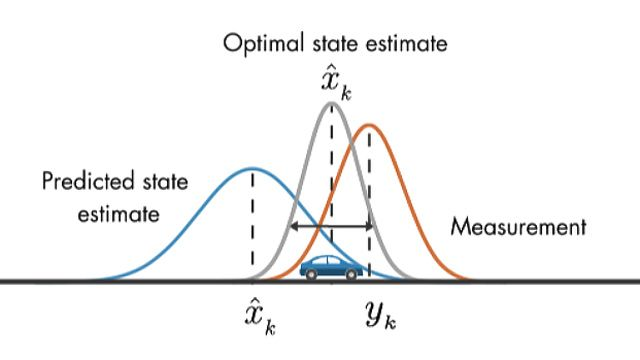
\includegraphics[width=1.0\linewidth]{images/kalman_2.jpg}
    \caption{Kalman filter prediction of the state using estimations. From: \cite{mathworks_kalman}.}
    \label{fig: Kalman filter prediction of the state using estimations.}
\end{figure}
\FloatBarrier\noindent

The Kalman filter follows a classical predict-update model, focusing on a single state variable: the vehicle’s velocity. The process and measurement uncertainty are encapsulated in the following variables:
\begin{itemize}
    \item Process variance Q: models the uncertainty in the vehicle’s motion (e.g., acceleration changes, jitter).
    \item Measurement variance R: represents the uncertainty in each self-speed estimation sample.
\end{itemize}

Where in real life the implementation can be represented as:
\begin{itemize}
    \item Estimated value: the current velocity estimate.
    \item Estimated error: the uncertainty (variance) of the current estimate.
\end{itemize}
At each new frame, a new self-speed estimation is used to update the Kalman filter which effects its output by a variable which is called Kalman Gain 'K':
\begin{equation}
K = \frac{\hat{P}}{\hat{P} + R}
\end{equation}
Where:
\begin{itemize}
    \item $\hat{P}$: predicted error variance
    \item $R$: measurement variance
\end{itemize}
This process allows the filter to balance trust between the incoming measurement and the current estimate. Over time, the filter becomes more confident, reducing the influence of noisy measurements.

Thus, the incorporation of the Kalman filter in this project provides smoother, more reliable self-speed estimation, which enhances the performance of the following dynamic filtering stage.

\begin{figure}[!htbp]
    \centering
    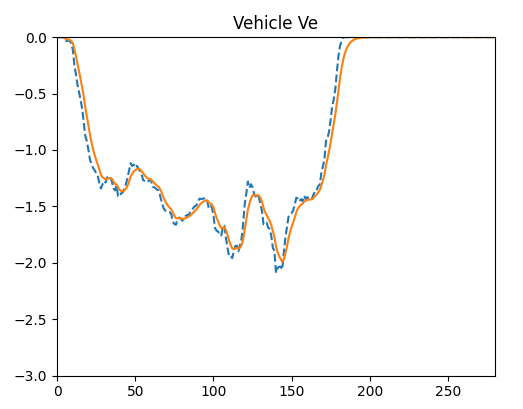
\includegraphics[width=1.0\linewidth]{images/kalman.png}
    \caption{Raw self-speed vs. self-speed after Kalman filter.}
    \label{fig: Test vehicle actual speed vs estimated speed.}
\end{figure}